% !TeX root = ../proyecto.tex

\chapter{Desarrollo Experimental}\label{ch:desarrollo-experimental}
En este capítulo se exponen los experimentos realizados, los ajustes implementados en los algoritmos y los resultados
obtenidos en los distintos escenarios evaluados.
El objetivo principal fue analizar el rendimiento de los modelos entrenados con conjuntos de datos reducidos,
seleccionados mediante algoritmos meméticos y evolutivos.

\section{Datasets utilizados}\label{sec:datasets}
En el aprendizaje profundo, los datasets son colecciones de datos etiquetados o no etiquetados que se utilizan para
entrenar modelos.
Estos conjuntos de datos contienen ejemplos organizados que representan la entrada para el modelo y, en muchos casos,
también las etiquetas correspondientes que indican la salida deseada.
Los datasets varían en tamaño, calidad y tipo, dependiendo de la tarea a resolver, como la clasificación de imágenes,
el reconocimiento de patrones o la predicción de series temporales.


A continuación, se van a explicar cada uno de los Datasets que se han utilizado en el desarrollo del proyecto.

\newpage

\subsection{Rock, Paper, Scissors (Piedra, Papel, Tijera)}\label{subsec:rock-paper-scissors}
\textbf{Rock, Paper, Scissors}~\cite{RockPaperScissors} es un conjunto de datos creado por Laurence Moroney
que se utiliza para la clasificación de imágenes de manos representando los gestos de `piedra', `papel' y `tijeras'.

\begin{figure}[H]
    \centering
    \begin{subfigure}[t]{0.3\textwidth}
        \centering
        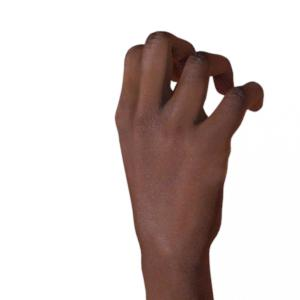
\includegraphics[width=\linewidth]{imagenes/dataset_examples/rock.jpg}
        \caption*{Rock}
    \end{subfigure}
    \begin{subfigure}[t]{0.3\textwidth}
        \centering
        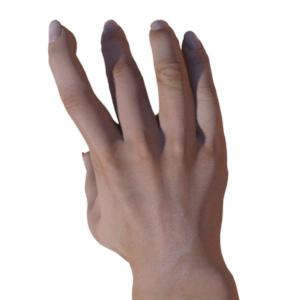
\includegraphics[width=\linewidth]{imagenes/dataset_examples/paper.jpg}
        \caption*{Paper}
    \end{subfigure}
    \begin{subfigure}[t]{0.3\textwidth}
        \centering
        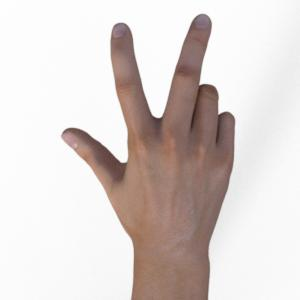
\includegraphics[width=\linewidth]{imagenes/dataset_examples/scissors.jpg}
        \caption*{Scissors}
    \end{subfigure}
    \caption{Ejemplos de imágenes del dataset Rock, Paper, Scissors}
    \label{fig:ejemplos-rps}
\end{figure}

En la figura~\ref{fig:ejemplos-rps} se han mostrado una imagen de cada una de las clases del dataset Rock, Paper, Scissors,
para que se pueda observar la similitud entre las distintas clases.

\subsubsection{Estructura del Dataset}
El conjunto de datos contiene aproximadamente 2,500 imágenes, distribuidas en tres categorías: piedra, papel y tijeras.
Las imágenes están en color y tienen un tamaño de 300x300 píxeles.

\begin{figure}[ht]
    \centering
    \begin{forest}mydirstyle
        [RPS
            [train
                    [rock
                            [image1.jpg]
                            [image2.jpg]
                            [\dots]
                    ]
                    [paper
                            [image1.jpg]
                            [image2.jpg]
                            [\dots]
                    ]
                    [scissors
                            [image1.jpg]
                            [image2.jpg]
                            [\dots]
                    ]
            ]
            [test (originalmente valid)
                [rock]
                    [paper]
                    [scissors]
            ]
            [valid (originalmente test)
                [rock]
                    [paper]
                    [scissors]
            ]
        ]
    \end{forest}
    \caption{Estructura de carpetas del dataset Rock, Paper, Scissors}
    \label{fig:estructura-rps}
\end{figure}


Como se puede observar en la Figura~\ref{fig:estructura-rps}, las imágenes están organizadas en directorios según su función en el entrenamiento
(entrenamiento, validación o prueba) y, dentro de cada partición, se dividen a su vez por clases del dataset.

\subsubsection{Formato de los Datos}
Las imágenes están en formato JPEG (\texttt{.jpg}).
Para su procesamiento, se han aplicado técnicas de preprocesamiento
adaptadas a los requerimientos del modelo.

\subsubsection{Uso del Dataset}
Este dataset se ha utilizado para evaluar el rendimiento del modelo en un problema de clasificación de imágenes con
múltiples clases, pero siendo un dataset sencillo y con un número de clases pequeño.
Además, permite explorar la eficacia de los algoritmos meméticos en un entorno más cercano al reconocimiento de objetos.

\subsubsection{Correcciones en la División de Datos}
Según la nota observada en el README del dataset:
\begin{quote}
    \textit{Note: in the source, Laurence calls ``validation'' as the ``test'', and ``test'' the ``validation''.}
\end{quote}
se han renombrado las particiones de \texttt{test} y \texttt{valid} para que correspondan correctamente con sus
propósitos.

\subsubsection{Licencia y uso}
Este conjunto de datos se distribuye bajo la licencia
\textbf{Creative Commons Attribution 4.0 International (CC BY 4.0)}, lo que permite su uso, modificación y distribución
con la condición de otorgar el crédito adecuado a los creadores originales~\cite{moroneyLaurenceMoroneyAI}.


\subsection{\texttt{PAINTING} (Art Images: Drawing/Painting/Sculptures/Engravings)}\label{subsec:painting}
El dataset \textbf{Art Images: Drawing/Painting/Sculptures/Engravings} es una colección de aproximadamente 9,000
imágenes organizadas en cinco categorías de arte: dibujos, pinturas, esculturas, grabados y arte iconográfico.

\begin{figure}[H]
    \centering
    \begin{subfigure}[t]{0.3\textwidth}
        \centering
        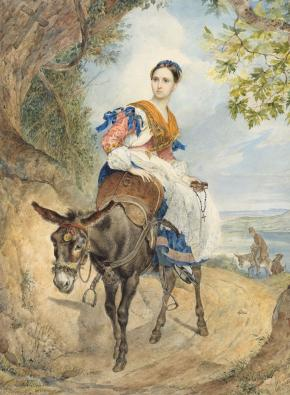
\includegraphics[width=\linewidth]{imagenes/dataset_examples/drawings.jpg}
        \caption*{Drawings}
    \end{subfigure}
    \begin{subfigure}[t]{0.3\textwidth}
        \centering
        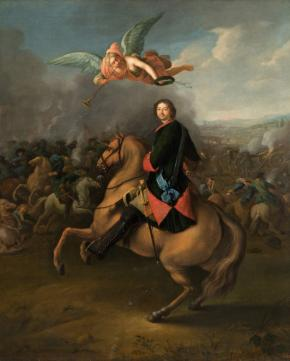
\includegraphics[width=\linewidth]{imagenes/dataset_examples/painting.jpg}
        \caption*{Painting}
    \end{subfigure}
    \begin{subfigure}[t]{0.3\textwidth}
        \centering
        
\includegraphics[width=\linewidth]{imagenes/dataset_examples/iconography.jpg}
        \caption*{Iconography}
    \end{subfigure}
    \begin{subfigure}[t]{0.3\textwidth}
        \centering
        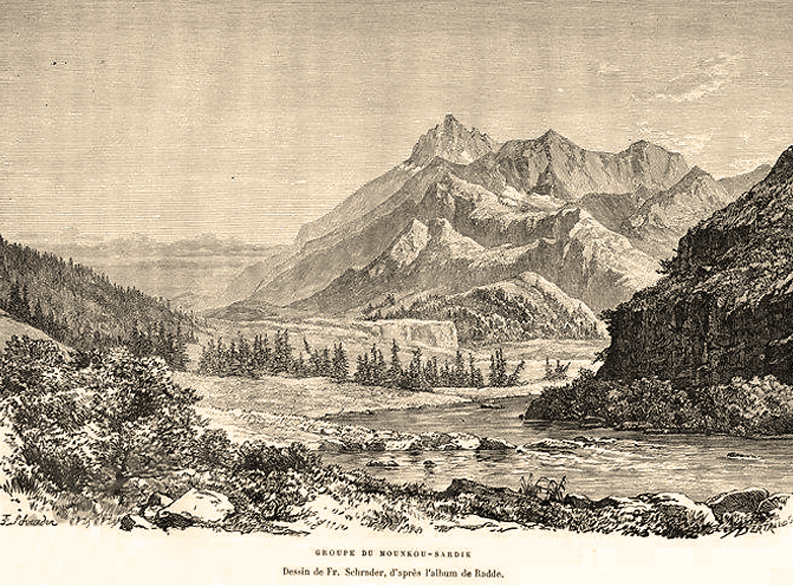
\includegraphics[width=\linewidth]{imagenes/dataset_examples/engraving.jpg}
        \caption*{Engraving}
    \end{subfigure}
    \begin{subfigure}[t]{0.3\textwidth}
        \centering
        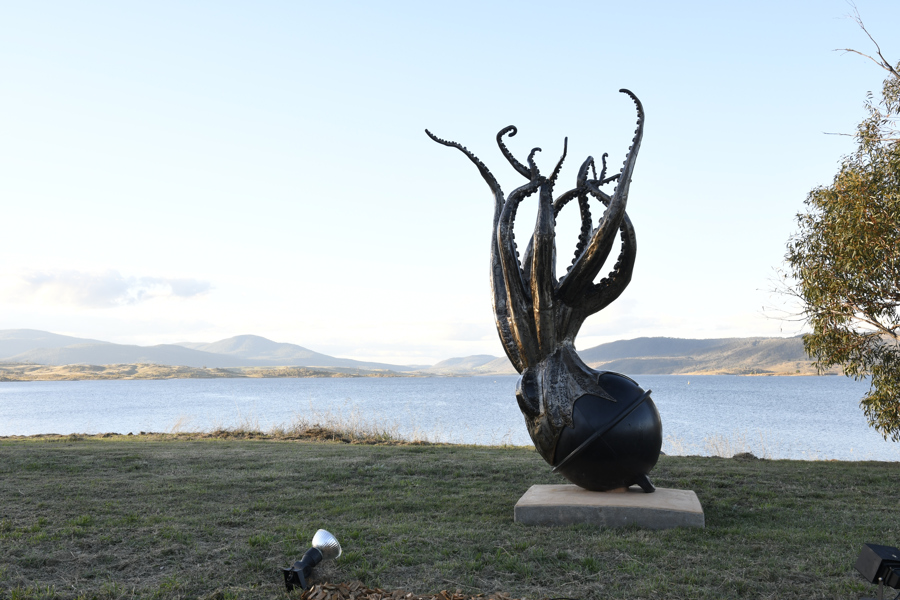
\includegraphics[width=\linewidth]{imagenes/dataset_examples/sculpture.jpg}
        \caption*{Sculpture}
    \end{subfigure}
    \caption{Ejemplos de clases en el dataset \texttt{PAINTING}}
    \label{fig:ejemplos-painting}
\end{figure}

En la figura~\ref{fig:ejemplos-painting} se han mostrado una imagen de cada una de las clases del dataset \texttt{PAINTING},
para que se pueda observar la variabilidad de las imágenes.

\subsubsection{Estructura del Dataset}
\begin{figure}[ht]
    \centering
    \begin{forest}mydirstyle
        [Dataset
            [Train (originalmente training\_set)
                [drawings
                            [image1.jpg]
                            [image2.jpg]
                            [\dots]
                    ]
                    [paintings
                            [image1.jpg]
                            [image2.jpg]
                            [\dots]
                    ]
                    [sculptures]
                    [engravings]
                    [iconography]
            ]
            [Test (originalmente validation\_set)
                [drawings]
                    [paintings]
                    [sculptures]
                    [engravings]
                    [iconography]
            ]
        ]
    \end{forest}
    \caption{Estructura de carpetas del dataset \texttt{PAINTING}}
    \label{fig:estructura-painting}
\end{figure}

Como se puede observar en la Figura~\ref{fig:estructura-painting}, las imágenes están organizadas en directorios según su categoría artística,
que en este caso corresponden a las distintas clases del dataset, previamente divididas en conjuntos de entrenamiento y prueba.

\subsubsection{Formato de los Datos}
Todas las imágenes están en formato JPEG (\texttt{.jpg}) y presentan variaciones en resolución y dimensiones.
Se han aplicado técnicas de preprocesamiento para homogenizar las características de las imágenes.

\subsubsection{Uso del Dataset}
Este dataset se ha utilizado para entrenar y evaluar modelos de clasificación de imágenes en un entorno diferente al
RPS\@.
Con este dataset, se ha comprobado el funcionamiento para evaluar los algoritmos con un dataset un poco mas complejo
que el RPS, con un par de clases más y con un número mayor de imágenes.

\subsubsection{Correcciones en la División de Datos}
Observando los tamaños de la división de los datos, y teniendo en cuenta que la divisón de los datos suele ser en train
y test, se ha decidido por renombrar las particiones de \texttt{valid} por \texttt{test} para que corresponda
correctamente con su propósito.
Y el set de validation lo he obtenido separando el set de train, normalmente haciendo una división 80\% test y 20\%
valid.

\subsubsection{Acceso al Dataset}
Inicialmente, el dataset se descargó desde Kaggle~\cite{OriginalArtImages}

Sin embargo, debido a la presencia de archivos innecesarios y algunas imágenes corruptas, se optó por una versión
limpia disponible en Kaggle~\cite{CleanedArtImages}.

\subsubsection{Licencia y Uso}
Antes de su uso, se revisaron los términos y condiciones establecidos en la página de Kaggle para asegurar el
cumplimiento con las licencias y restricciones aplicables.

\subsection{Comparación entre datasets}\label{subsec:comparacion-entre-datasets}
A continuación, se muestra una tabla resumen con las características más relevantes de los datasets utilizados.
Esta comparación permite entender mejor la complejidad relativa de cada conjunto y cómo pueden influir en el comportamiento de los algoritmos:

\begin{table}[H]
    \centering
    \resizebox{\textwidth}{!}{
        \begin{tabular}{|l|c|c|c|c|}
            \hline
            \textbf{Dataset}      & \textbf{Nº Imágenes} & \textbf{Nº Clases} & \textbf{Formato} & \textbf{Tamaño Imagen} \\
            \hline
            Rock, Paper, Scissors & \textasciitilde2.500 & 3                  & JPG              & 300×300 px             \\
            PAINTING              & \textasciitilde9.000 & 5                  & JPG              & Variable               \\
            \hline
        \end{tabular}
    }
    \caption{Resumen comparativo de los datasets utilizados}
    \label{tab:resumen-datasets}
\end{table}

La selección de estos dos datasets responde a la necesidad de evaluar los algoritmos meméticos en distintos niveles de complejidad.
El dataset \textbf{Rock, Paper, Scissors} se utilizó en las primeras fases del proyecto como punto de partida,
ya que ofrecía un entorno sencillo y controlado, con un número reducido de clases y una estructura equilibrada.
Esto permitió desarrollar las bases del sistema y probar las primeras versiones de los algoritmos de manera más ágil y con menor complejidad computacional.

Por su parte, el dataset \textbf{PAINTING} se empleó posteriormente para validar el comportamiento de los algoritmos en un entorno más exigente.
Al incluir cinco categorías de arte con distintos estilos visuales, este conjunto introdujo una mayor variabilidad tanto semántica como estructural,
lo que permitió evaluar la robustez y capacidad de generalización de las soluciones desarrolladas.


\section{Diseño de los experimentos}\label{sec:diseño-de-los-experimentos}
La fase experimental se organizó en varias etapas.
Inicialmente se optó por un dataset simple (\textit{Rock, Paper, Scissors}) para validar el funcionamiento general del sistema.
Posteriormente, se realizaron pruebas con datasets más exigentes.
Los experimentos se repitieron utilizando diferentes porcentajes iniciales de datos (10\%, 25\%, 50\% y 75\%)
para estudiar cómo afecta la cantidad de datos seleccionados al rendimiento del modelo.

Con el fin de asegurar la consistencia entre ejecuciones experimentales, se aplicaron las medidas de control de reproducibilidad
descritas en el \hyperref[sec:consideraciones-de-optimizacion]{Apartado~\ref*{sec:consideraciones-de-optimizacion}}.
Esto permitió comparar algoritmos en condiciones homogéneas, evitando variaciones indeseadas causadas por componentes aleatorios del entorno de ejecución.

En cada prueba, se realizaron 5 ejecuciones en paralelo, cada una utilizando una semilla distinta.
Esta estrategia permitió obtener resultados promedio más robustos frente a la aleatoriedad del proceso evolutivo, asegurando una mayor fiabilidad estadística.

Los apartados siguientes explican con mayor detalle el procedimiento adoptado para llevar a cabo dichas ejecuciones.


\section{Procedimiento de Ejecución y Evaluación}\label{sec:procedimiento-de-ejecucion-y-evaluacion}
Para garantizar la consistencia y objetividad en la comparación entre algoritmos, se diseñó un procedimiento experimental sistemático y replicable.
Cada ejecución se realizó bajo las mismas condiciones computacionales y utilizando los mismos parámetros base,
salvo en aquellos casos en que se deseaba estudiar una variación concreta, como los distintos porcentajes iniciales o el uso de metaheurísticas con porcentajes libres.

\subsection{Métricas de Evaluación}\label{sec:metricas-de-evaluacion}
Para evaluar el rendimiento de los modelos se utilizaron métricas estándar como \textbf{accuracy}, \textbf{precisión}, \textbf{recall} y \textbf{F1-score},
calculadas sobre el conjunto de validación tras cada evaluación.
Para una definición formal de estas métricas, véase el \hyperref[sec:metricas-evaluacion]{Apartado~\ref*{sec:metricas-evaluacion}}.

Estas métricas fueron calculadas utilizando las funciones de \texttt{scikit-learn}, a partir de las predicciones del modelo y las etiquetas
reales correspondientes a los subconjuntos de imágenes seleccionados por cada algoritmo.

\subsection{Evaluaciones por Ejecución}\label{sec:evaluaciones-por-ejecucion}
Se buscó un equilibrio entre la cantidad de evaluaciones y el tiempo de ejecución, permitiendo una exploración suficiente del espacio de soluciones sin comprometer la eficiencia computacional.
Por ello, cada algoritmo fue configurado para realizar un máximo de 100 evaluaciones por ejecución,
independientemente del tipo de algoritmo utilizado, con el fin de mantener la equidad comparativa.

Cada evaluación consistía en generar un subconjunto de datos, entrenar el modelo correspondiente (ResNet50 o MobileNetV2),
y calcular su \textit{fitness} de acuerdo con las métricas mencionadas.

El número de evaluaciones sin mejora también fue monitorizado para aplicar criterios de parada anticipada,
explicados previamente en el \hyperref[sec:consideraciones-de-optimizacion]{Apartado~\ref*{sec:consideraciones-de-optimizacion}},
reduciendo así el tiempo computacional en caso de estancamiento.

\subsubsection{Visualización de resultados}\label{subsec:visualizacion-de-resultados}
Para facilitar la comparación entre algoritmos, a lo largo de este capítulo se incluyen representaciones gráficas de los resultados obtenidos mediante \textbf{boxplots} y \textbf{barplots}.
Ambos tipos de gráficos permiten visualizar el comportamiento global de cada algoritmo a partir de múltiples ejecuciones con distintas semillas.

\textbf{Los boxplots} (diagramas de caja) muestran la distribución estadística de los valores obtenidos.
En la Figura~\ref{fig:boxplot-explicado} se presenta un ejemplo anotado que ilustra las distintas partes de este tipo de gráfico.
La línea central de la caja representa la \textbf{mediana},
mientras que los bordes inferior y superior corresponden al \textbf{primer cuartil} (Q1) y \textbf{tercer cuartil} (Q3), respectivamente.
La diferencia entre ellos define el \textbf{rango intercuartílico} (\textit{IQR}), que contiene el 50\% central de los valores.
Las líneas que se extienden desde la caja (conocidas como \textit{bigotes}) alcanzan típicamente hasta 1.5 veces el IQR.
Los puntos que quedan fuera de ese rango se consideran \textbf{valores atípicos}, lo que permite detectar ejecuciones excepcionales.
Esta representación es especialmente útil para comparar la tendencia central, la dispersión y la estabilidad de los resultados obtenidos por los distintos algoritmos.

\begin{figure}[H]
    \centering
    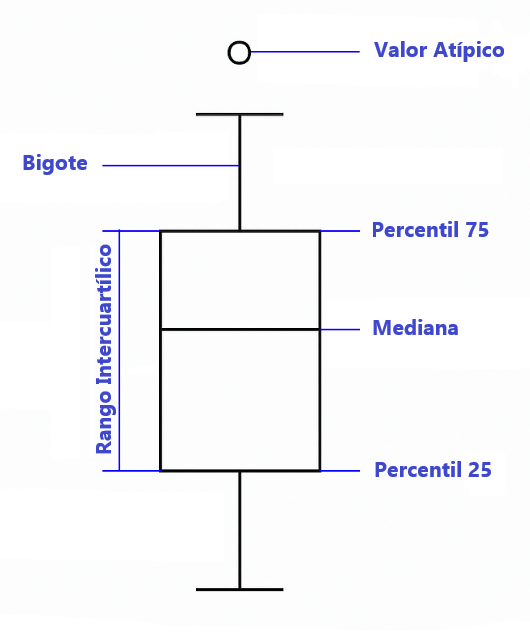
\includegraphics[width=0.45\textwidth]{imagenes/boxplot-explicado}
    \caption{Ejemplo de boxplot explicado.}
    \label{fig:boxplot-explicado}
\end{figure}

\textbf{Los barplots} (gráficos de barras), por su parte, se emplean para representar valores agregados como medias o proporciones,
y son útiles para observar cómo varía una métrica concreta entre distintos algoritmos, modelos o configuraciones.

\subsection{Repeticiones y Semillas}\label{sec:repeticiones-y-semillas}
Con el objetivo de obtener resultados estadísticamente significativos y reducir el efecto de la aleatoriedad,
cada configuración experimental fue ejecutada 5 veces, utilizando 5 semillas distintas.
Los resultados presentados en las tablas y gráficos corresponden a la media de esas ejecuciones,
junto con medidas de dispersión cuando procede, como los boxplots.

Cabe destacar que, en el caso de los boxplots, en lugar de representar la media de las 5 ejecuciones por configuración,
se optó por incluir todos los valores individuales obtenidos con las distintas semillas.
Esta decisión permite visualizar una distribución más realista del comportamiento de cada algoritmo,
resaltando mejor la mediana, así como los valores máximos y mínimos alcanzados durante las ejecuciones.

\subsection{Tiempos de Ejecución}\label{sec:tiempos-de-ejecucion}
Cada evaluación implicaba entrenar un modelo desde cero, por lo que los tiempos de ejecución fueron considerables.
Por ejemplo, una ejecución completa con 100 evaluaciones podía tardar entre 30 minutos y 2 horas,
dependiendo del algoritmo y del modelo utilizado.

Los algoritmos más complejos, como el memético o las versiones con reinicio poblacional,
requerían un mayor tiempo de ejecución debido a las operaciones adicionales de mejora local o regeneración de población.


\section{Evaluación con el conjunto completo}\label{sec:evaluacion-con-el-conjunto-completo}
Como punto de partida, se evaluó el rendimiento de los modelos convolucionales entrenados con el 100\% del conjunto de datos.
Esta prueba sirve como referencia para contrastar los resultados obtenidos mediante las técnicas de reducción aplicadas posteriormente.
Se utilizó tanto ResNet50 como MobileNetV2, y se midieron métricas como accuracy, precisión, recall y F1-score sobre el conjunto de validación.

\begin{table}[htp]
    \centering
    \resizebox{\textwidth}{!}{
        \begin{tabular}{lp{2cm}lp{2cm}p{2cm}p{2cm}p{2cm}p{2.2cm}}
            \toprule
            \textbf{Porcentaje Inicial} & \textbf{Duración}     & \textbf{Accuracy (Avg)} &
            \textbf{Precision (Avg)}    & \textbf{Recall (Avg)} & \textbf{F1-score (Avg)} &
            \textbf{Evaluaciones Realizadas}                                                                                \\
            \midrule
            100                         & 00:02:42              & 87,90\%                 & 88,96\% & 87,90\% & 87,81\% & 1 \\
            \bottomrule
        \end{tabular}
    }
    \caption{Resultados de ResNet50 entrenado con el 100\% del conjunto de datos.}
    \label{tab:resultados-100-resnet50}
\end{table}

Los resultados en la tabla~\ref{tab:resultados-100-resnet50} obtenidos representan el rendimiento máximo alcanzable en condiciones ideales,
sin reducción de datos, lo que permite establecer un techo de rendimiento frente al cual comparar las demás técnicas.


\section{Evaluación del enfoque aleatorio}\label{sec:evaluacion-enfoque-aleatorio}
El segundo experimento consistió en aplicar una selección aleatoria de ejemplos para distintos porcentajes iniciales de datos (10\%, 25\%, 50\% y 75\%).
Este enfoque, descrito en el \hyperref[sec:algoritmo-aleatorio]{Apartado~\ref*{sec:algoritmo-aleatorio}}, sirvió como línea base para evaluar la eficacia de los enfoques metaheurísticos.

\begin{figure}[!h]
    \centering
    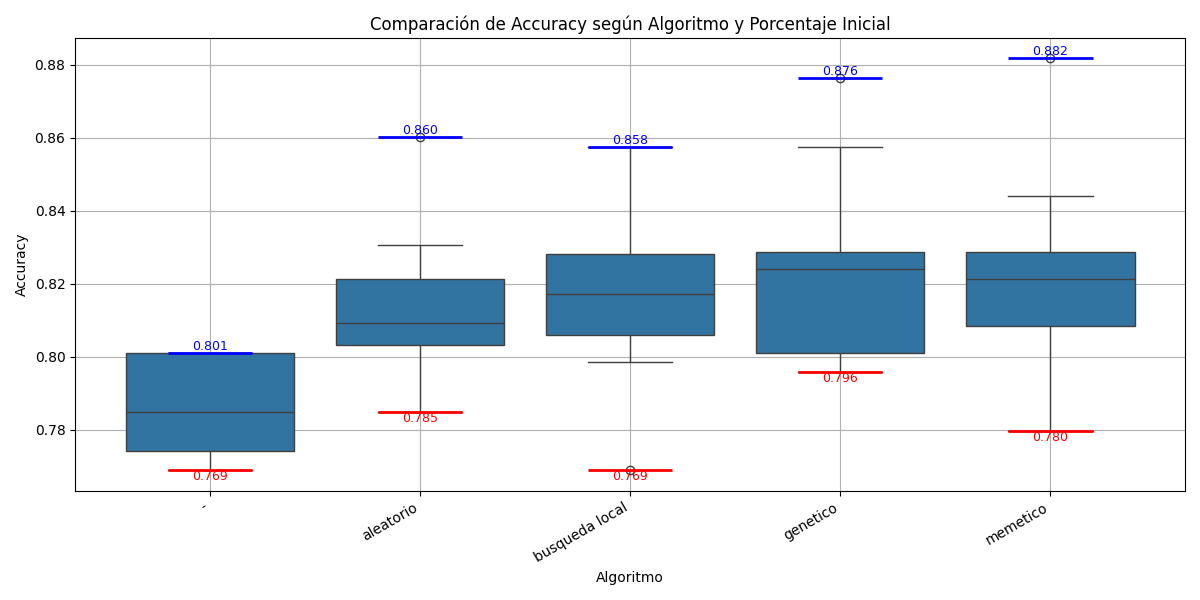
\includegraphics[width=0.95\textwidth]{imagenes/mobilenet-BOXPLOT-generacion-inicial}
    \caption{Boxplot comparando el \textit{accuracy} alcanzado por cada algoritmo de los iniciales.}
    \label{fig:resnet-boxplot-generacion-inicial}
\end{figure}

\colorbox{yellow}{Falta modificar la tabla~\ref{fig:resnet-boxplot-generacion-inicial} para que compare el 100\% con el aleatorio de resnet y ajustar analisis si es necesario.}
\colorbox{yellow}{Falta añadir tabla comparando resultados por porcentajes iniciales.}

Tal como se observa en el boxplot generado (\hyperref[fig:resnet-boxplot-generacion-inicial]{Figura~\ref*{fig:resnet-boxplot-generacion-inicial}}),
como era de esperar, presenta una alta dispersión, pero el rendimiento es mejor que el resultado con el 100\% del dataset.
Ademas, en esta otra tabla [tabla comparando resultados por porcentajes iniciales] los resultados mejoran de forma proporcional al incremento del porcentaje de imágenes seleccionadas.
Este comportamiento se justifica por la ausencia de una estrategia que guíe la selección de datos, lo que da lugar a conjuntos de entrenamiento inconsistentes y
resalta la necesidad de aplicar técnicas más sofisticadas para obtener resultados consistentes con menores volúmenes de datos.


\section{Comparación entre modelos convolucionales}\label{sec:comparacion-modelos-convolucionales}
Antes de analizar los algoritmos de reducción, se comparó el comportamiento de los modelos \textbf{ResNet50} y \textbf{MobileNetV2} bajo las mismas condiciones de entrenamiento y subconjuntos aleatorios.

\begin{table}[H]
    \centering
    \resizebox{\textwidth}{!}{
        \begin{tabular}{lp{2cm}lp{2cm}p{2cm}p{2cm}p{2cm}p{2.2cm}}
            \toprule
            \textbf{Algoritmo}       & \textbf{Porcentaje Inicial} & \textbf{Duración}       & \textbf{Accuracy (Avg)} &
            \textbf{Precision (Avg)} & \textbf{Recall (Avg)}       & \textbf{F1-score (Avg)} &
            \textbf{Evaluaciones Realizadas}                                                                                                               \\
            \midrule
            \multicolumn{8}{l}{\textbf{Modelo ResNet50}}                                                                                                   \\
            \midrule
            aleatorio                & 10                          & 00:45:08                & 76,55\%                 & 81,80\% & 76,55\% & 76,25\% & 100 \\
            aleatorio                & 20                          & 01:10:27                & 81,77\%                 & 84,70\% & 81,77\% & 81,59\% & 100 \\
            aleatorio                & 50                          & 02:24:49                & 87,14\%                 & 88,09\% & 87,14\% & 86,97\% & 100 \\
            aleatorio                & 100                         & 00:02:42                & 87,90\%                 & 88,96\% & 87,90\% & 87,81\% & 1   \\
            \midrule
            \multicolumn{8}{l}{\textbf{Modelo MobileNet}}                                                                                                  \\
            \midrule
            aleatorio                & 10\%                        & 00:29:29                & 72,31\%                 & 76,40\% & 72,31\% & 69,62\% & 100 \\
            aleatorio                & 20\%                        & 00:50:36                & 76,48\%                 & 78,82\% & 76,48\% & 75,58\% & 100 \\
            aleatorio                & 50\%                        & 01:54:09                & 75,56\%                 & 79,72\% & 75,56\% & 74,67\% & 100 \\
            -                        & 100\%                       & 00:03:16                & 78,60\%                 & 81,55\% & 78,60\% & 77,68\% & 1   \\
            \bottomrule
        \end{tabular}
    }
    \caption{Comparativa de resultados de la generación inicial utilizando el algoritmo \textbf{aleatorio} con los modelos \textbf{ResNet50} y \textbf{MobileNet}.}
    \label{tab:resnet50-vs-mobilenet}
\end{table}

Los resultados de la tabla~\ref{tab:resnet50-vs-mobilenet} muestran que ResNet50 mostró consistentemente mejores métricas,
aunque a costa de mayores tiempos de entrenamiento.
Por su parte, MobileNetV2 demostró ser más eficiente, resultando útil para entornos con restricciones computacionales.

Esta comparación justificó la elección de MobileNet como modelo principal en el resto de los experimentos,
dada su superior eficiencia en términos de tiempo y recursos, posibilitando la facilidad de realizar múltiples pruebas en un tiempo razonable.


\section{Estudio de la búsqueda local}\label{sec:estudio-busqueda-local}
Como se describió en el apartado correspondiente (ver \hyperref[sec:algoritmo-busqueda-local]{Sección~\ref*{sec:algoritmo-busqueda-local}}),
la búsqueda local permite mejorar progresivamente una solución inicial mediante pequeñas modificaciones guiadas por el rendimiento.
En este apartado se evalúa su efectividad como alternativa más estructurada frente al enfoque aleatorio, pero sin llegar a la complejidad de los algoritmos evolutivos.
Su inclusión busca analizar hasta qué punto una estrategia simple pero guiada puede generar subconjuntos de datos más representativos y consistentes.

\begin{figure}[H]
    \centering
    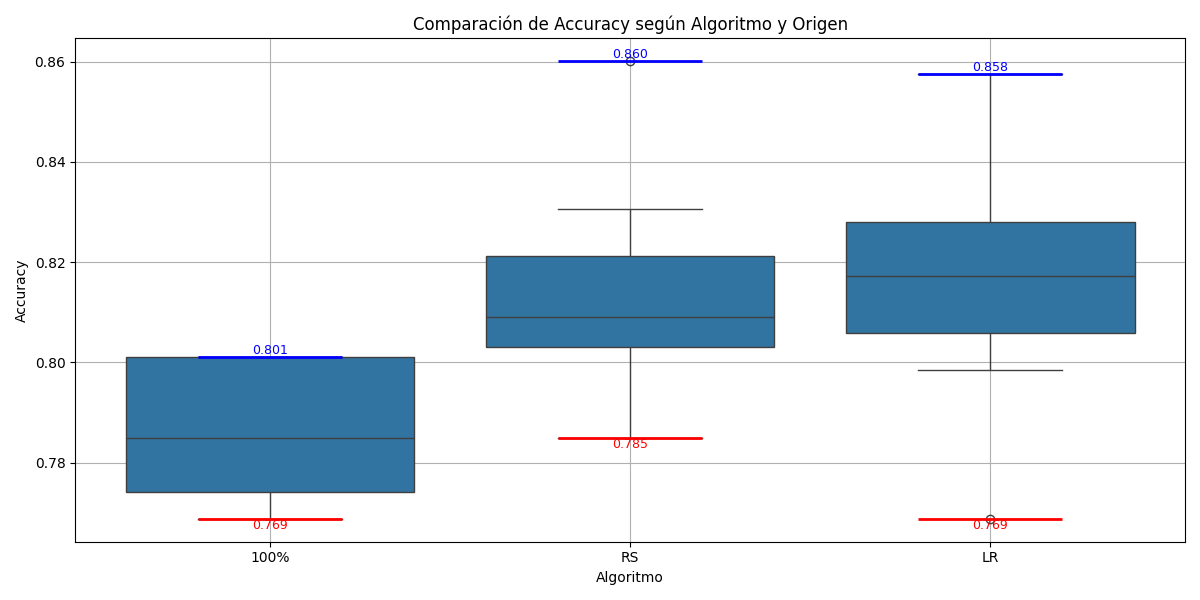
\includegraphics[width=1\textwidth]{imagenes/evaluaciones/comparacion_aleatorio-bl}
    \caption{Boxplot comparando el algoritmo aleatorio con la búsqueda local usando \textit{accuracy}.}
    \label{fig:aleatorio-vs-busqueda-local}
\end{figure}

En la Figura~\ref{fig:aleatorio-vs-busqueda-local} se muestran los resultados mediante un boxplot que permite observar
la distribución completa de valores obtenidos en las distintas ejecuciones.

Se puede apreciar que el algoritmo de búsqueda local mejora claramente la mediana del \textit{accuracy} respecto al enfoque aleatorio.
Mientras que el enfoque aleatorio se sitúa en torno a una mediana de 0.787, la búsqueda local alcanza una mediana superior, próxima a 0.818.
Esta diferencia refleja una mayor capacidad del algoritmo local para generar subconjuntos más representativos y eficaces.

Además, los valores máximos alcanzados por ambos algoritmos son similares (en torno a 0.858-0.860),
pero la búsqueda local muestra una dispersión más acotada hacia valores altos, lo que sugiere mayor estabilidad en sus resultados.
En cambio, el algoritmo aleatorio presenta una mayor dispersión hacia valores bajos y una mayor sensibilidad a la aleatoriedad de las selecciones,
como se evidencia en su menor valor mínimo (0.769 frente a 0.785 en búsqueda local).

Esto pone de manifiesto que, aunque el algoritmo aleatorio puede ocasionalmente alcanzar buenos resultados,
la búsqueda local ofrece una mejor consistencia y fiabilidad, con menos varianza entre ejecuciones y una tendencia general a obtener subconjuntos de entrenamiento más efectivos.


\section{Estudiando la mejora metaheurística}\label{sec:estudio-mejora-metaheuristica}
Con el objetivo de superar las limitaciones observadas (como el riesgo de estancamiento o la exploración poco estructurada del espacio de soluciones)
se incorporó un enfoque evolutivo más completo: el algoritmo genético, descrito en la Sección~\ref{sec:genetico-v1}, el cual sirvió como punto de partida para explorar la
aplicación de estrategias metaheurísticas en la selección de subconjuntos representativos de imágenes.
Su estructura evolutiva, basada en selección por torneo, cruce e incorporación de mutación,
ofrecía ya desde sus primeras versiones una capacidad superior para generalizar, en comparación con métodos más simples como la búsqueda local.

\begin{figure}[H]
    \centering
    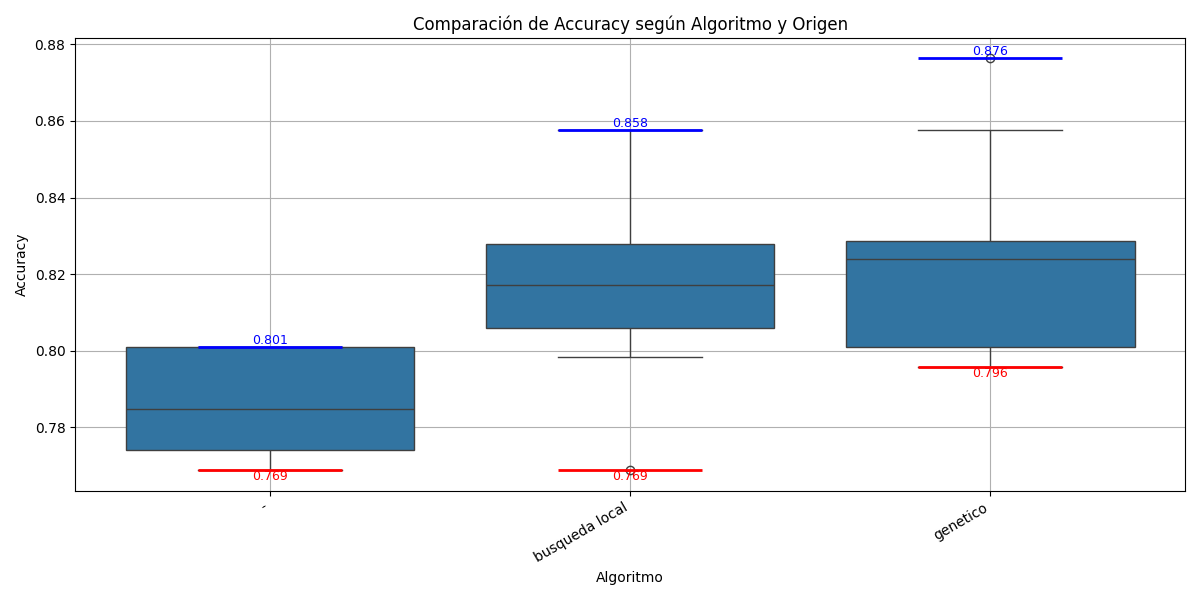
\includegraphics[width=1\textwidth]{imagenes/evaluaciones/comparacion_bl-gen_v1}
    \caption{Boxplot comparando la búsqueda local con el algoritmo genético v1 usando \textit{accuracy}.}
    \label{fig:bl-vs-gen-v1}
\end{figure}

Tal como se observa en la Figura~\ref{fig:bl-vs-gen-v1}, el algoritmo genético consigue una \textbf{mediana de \textit{accuracy}} más alta que la búsqueda local,
reflejando un rendimiento medio más consistente.
Además, presenta un valor máximo superior (alcanza hasta \textbf{0.876}), lo que evidencia su mayor potencial para encontrar soluciones de alta calidad.

No obstante, también se aprecia una ligera mayor dispersión en los resultados del algoritmo genético, particularmente hacia los valores bajos.
Esto indica que, pese a su capacidad exploratoria, el genético puede generar soluciones poco efectivas si no se controlan adecuadamente ciertos operadores como el cruce o la mutación.
De hecho, su valor mínimo (\textbf{0.796}) es superior al de la búsqueda local en esta comparativa, pero deja margen para mejoras en la presión selectiva o en mecanismos que eviten estancamientos.

\colorbox{yellow}{¿Sobra el siguiente apartado?}
La búsqueda local, por su parte, mantiene un comportamiento más estable, aunque con una mediana ligeramente inferior.
Su distribución es más concentrada y limitada en el extremo superior, lo que evidencia su carácter más explotador pero con menor capacidad para alcanzar soluciones óptimas globales.

Estos resultados sirvieron como evidencia empírica para continuar desarrollando nuevas versiones del algoritmo genético,
incorporando mejoras específicas en sus operadores con el fin de aprovechar su capacidad exploratoria y, al mismo tiempo, mitigar sus limitaciones.

\section{Modificando el operador de cruce}\label{sec:incorporacion-cruce}
La primera mejora introducida al algoritmo genético consistió en reemplazar el cruce aleatorio por un cruce ponderado,
donde se prioriza la contribución del progenitor con mayor \textit{fitness}.
Además, se incorporó una estrategia selectiva que conserva únicamente el mejor de los dos hijos generados en cada cruce.
Ambos cambios, explicados en detalle en la \hyperref[sec:genetico-v2]{Sección~\ref*{sec:genetico-v2}},
buscan aumentar la presión evolutiva y acelerar la convergencia hacia soluciones de mayor calidad,
evitando así que soluciones mediocres se propaguen innecesariamente en la población.

\begin{figure}[H]
    \centering
    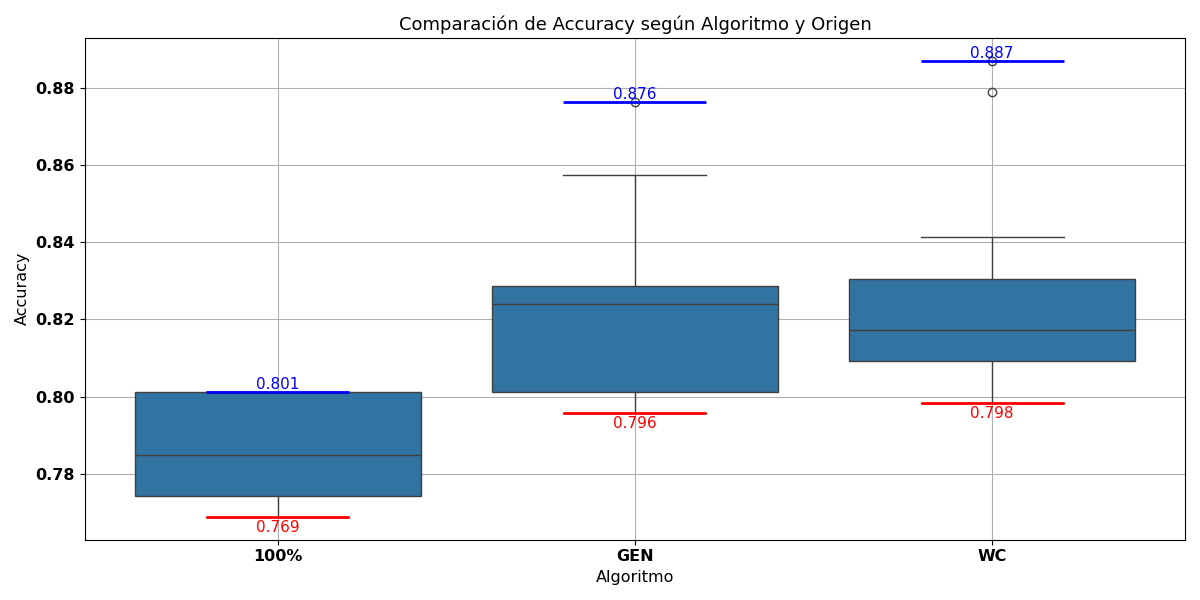
\includegraphics[width=1\textwidth]{imagenes/evaluaciones/operador-de-cruce}
    \caption{Boxplot de \textit{accuracy} para el genético, versión con cruce ponderado y dataset completo.}
    \label{fig:cruce_ponderado}
\end{figure}

Tal como se observa en la Figura~\ref{fig:cruce_ponderado}, esta modificación produjo una mejora clara en la calidad y estabilidad de los resultados.
La versión con cruce ponderado (etiquetada como \texttt{genetico2}) alcanza un valor máximo atípico superior (\textbf{0.887}),
aunque presenta una mediana más baja que la versión básica.

Pero por otra parte, se aprecia una ligera reducción en la dispersión de los valores inferiores,
con un mínimo de \textbf{0.798} frente al \textbf{0.796} en la versión anterior, lo que sugiere una mayor consistencia.
Aunque el IQR (\hyperref[subsec:visualizacion-de-resultados]{Rango Intercuartílico}) sigue siendo amplio,
la acumulación de valores más cercanos al rango superior refleja una convergencia evolutiva más enfocada y menos dependiente del azar.

En conjunto, esta mejora en el cruce no solo permitió una transferencia más eficiente de características ventajosas,
sino que también incrementó la presión selectiva sobre la calidad de las soluciones.
Esto se tradujo en un comportamiento más robusto, menos propenso a resultados erráticos y con una mayor capacidad de exploración dirigida del espacio de soluciones.


\section{Modificación del operador de mutación}\label{sec:modificacion-mutacion}
A partir de los resultados obtenidos con el algoritmo con cruce ponderado, se evaluó una nueva versión en la que se introdujo una mutación adaptativa
(ver \hyperref[sec:genetico-mutacion]{Sección~\ref*{sec:genetico-mutacion}}).
A diferencia de la versión original con tasa fija, esta estrategia ajusta el número de intercambios en función del tamaño del subconjunto mutado,
lo que permite una mayor flexibilidad en escenarios de diferente escala.

\begin{figure}[H]
    \centering
    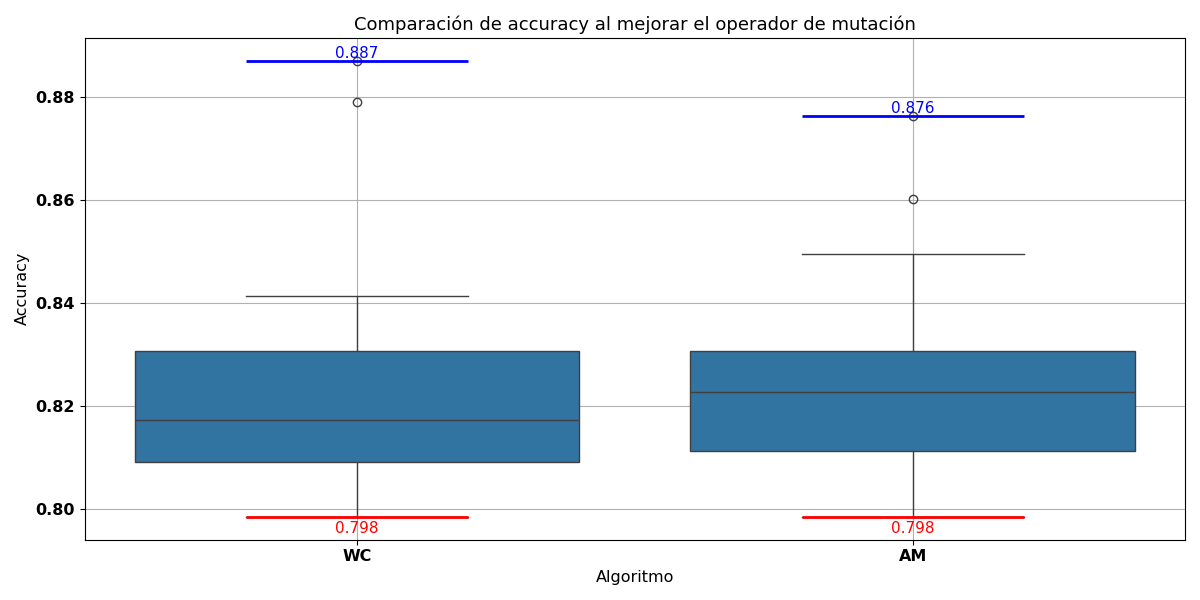
\includegraphics[width=1\textwidth]{imagenes/evaluaciones/mutacion-adaptativa}
    \caption{Comparación de \textit{accuracy} entre el algoritmo con cruce ponderado (\textit{genetico2}) y su versión con mutación adaptativa (\textit{genetico2\_2}).}
    \label{fig:mutacion-adaptativa}
\end{figure}

Como se observa en la Figura~\ref{fig:mutacion-adaptativa}, ambos algoritmos alcanzan un rendimiento similar en términos de mediana y valores extremos,
con una ligera ventaja de la versión original (\texttt{genetico2}) en el valor máximo de \textit{accuracy} (\textbf{0.887} frente a \textbf{0.876}).
Sin embargo, la versión con mutación adaptativa (\texttt{genetico2\_2}) muestra una distribución más compacta en la parte central,
con menos dispersión hacia valores bajos del IQR, lo que sugiere una mejora en la consistencia entre ejecuciones.

Además, la versión con mutación adaptativa presenta un Q4 más elevado, es decir, su \textit{bigote superior} abarca valores superiores a los de la versión original.
Esto indica que, aparte de que la mediana sea un poco superior, un mayor número de ejecuciones alcanzan rendimientos más altos de forma consistente,
reforzando la idea de que esta variante promueve una evolución más estable y con mayor concentración de soluciones de calidad en el tramo alto del rendimiento.

Este resultado refleja que, aunque la mutación adaptativa no produce una mejora radical en precisión media,
sí contribuye a una evolución más controlada y robusta, reduciendo la probabilidad de degradaciones abruptas.
Además, su comportamiento flexible la hace más adecuada en contextos donde el tamaño del subconjunto varía,
evitando configuraciones subóptimas impuestas por una tasa fija.

Aunque el valor máximo de \textit{accuracy} se mantiene en niveles similares, la ganancia está en la consistencia y la eficiencia exploratoria,
ya que se adapta automáticamente al contexto sin requerir ajustes manuales para diferentes tamaños de subconjuntos.
En conjunto, esta mejora refuerza la capacidad del algoritmo para mantener el equilibrio entre exploración y explotación durante el proceso evolutivo.


\section{Incorporación del reinicio poblacional}\label{sec:incorporacion-reinicio-poblacional}
La Versión3 del algoritmo genético (ver \hyperref[sec:genetico-v3]{Sección~\ref*{sec:genetico-v3}})
introduce una lógica de reinicio poblacional diseñada para evitar estancamientos evolutivos.
El algoritmo monitoriza el rendimiento del segundo mejor individuo, y si este no mejora durante dos generaciones consecutivas,
se aplica un reinicio parcial que conserva únicamente al mejor individuo de la población.

\begin{figure}[H]
    \centering
    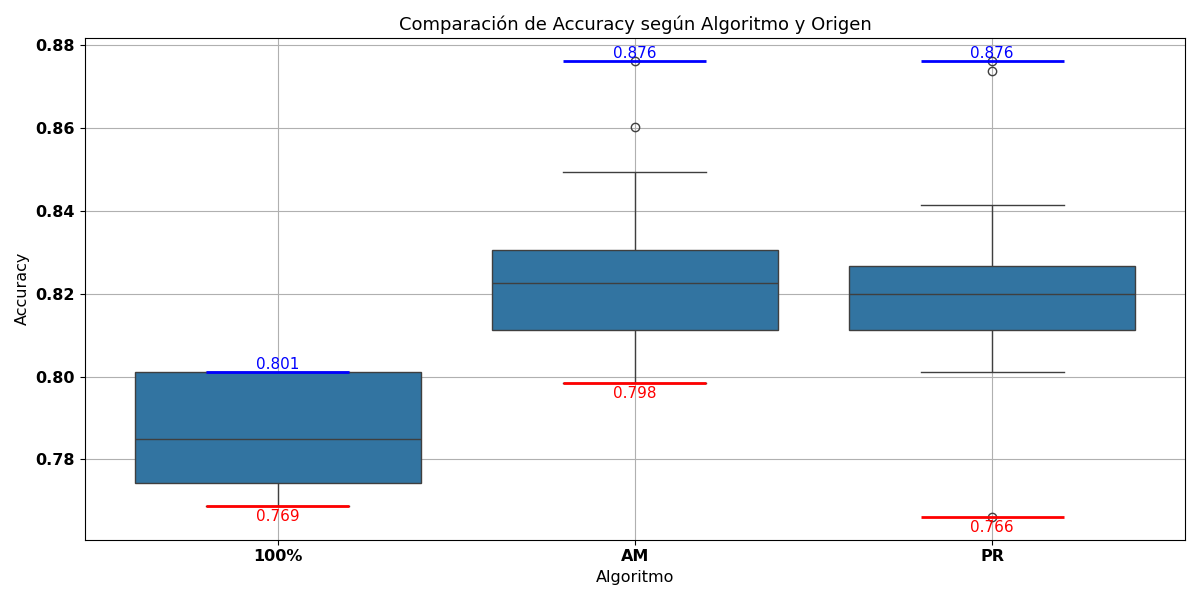
\includegraphics[width=1\textwidth]{imagenes/evaluaciones/reinicio-poblacional}
    \caption{Comparación de \textit{accuracy} entre el algoritmo genético con mutación adaptativa (genetico2\_2) y con reinicio poblacional (genetico3).}
    \label{fig:reinicio_poblacional}
\end{figure}

Tal como se observa en la Figura~\ref{fig:reinicio_poblacional}, los resultados muestran que la incorporación del reinicio no se tradujo en una mejora tangible del rendimiento.
La mediana de \texttt{genetico3} permanece prácticamente inalterada respecto a \texttt{genetico2\_2} (incluso ligeramente inferior),
y aunque el valor mínimo es inferior (\textbf{0.766} frente a \textbf{0.798}), no se aprecia un incremento en el valor máximo ni una reducción clara en la dispersión.

Esto sugiere que, al menos en este contexto experimental, el mecanismo de reinicio no logra mejorar la exploración del espacio de soluciones 
ni mitigar el estancamiento de forma eficaz.
En algunos casos, incluso puede introducir una pérdida prematura de diversidad, al regenerar de forma aleatoria parte de la población sin garantizar mejoras sustanciales.

\colorbox{yellow}{¿Añadir el párrafo de resumen?}
En resumen, aunque el reinicio poblacional es una estrategia teóricamente útil para escapar de óptimos locales,
su implementación en esta versión no logró aportar beneficios consistentes en términos de rendimiento.
Estos resultados invitan a reconsiderar su activación por defecto, o bien a explorar variantes más refinadas del mecanismo de reinicio.


\section{Incorporación de versiones libres}\label{sec:incorporacion-versiones-libres}
Como parte de la evolución de los algoritmos desarrollados, se propusieron versiones libres,
en las que el tamaño del subconjunto seleccionado no permanece fijo durante la ejecución, sino que puede ajustarse de forma dinámica.

Para evaluar esta flexibilidad, se generaron versiones libres de la búsqueda local y del algoritmo genético con cruce ponderado y mutación adaptativa, 
como modificación adicional, se introdujo un mecanismo al algoritmo de búsqueda local
en el que se seleccionaba de forma aletarioa el porcentaje inicial de imágenes a partir del cual se comenzaba a trabajar.


\begin{figure}[H]
    \centering
    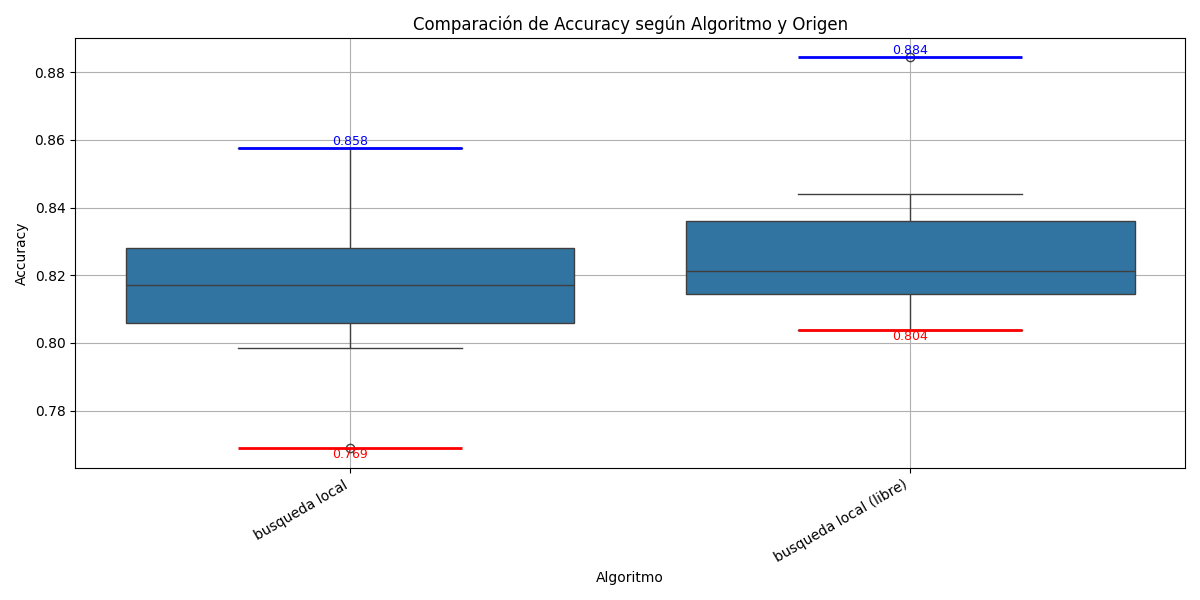
\includegraphics[width=0.9\textwidth]{imagenes/evaluaciones/libres/comparacion_bl}
    \caption{Comparación de \textit{accuracy} entre la búsqueda local estándar y su versión libre.}
    \label{fig:bl_libre}
\end{figure}

En la Figura~\ref{fig:bl_libre} se observa que la versión libre de la búsqueda local mejora tanto la mediana 
como el valor máximo de \textit{accuracy} respecto a su versión original.
Presenta, además, una menor dispersión en los valores bajos y una mayor concentración de ejecuciones en torno al cuartil superior, 
lo que sugiere una mejora en la estabilidad del algoritmo.
Este comportamiento refleja que introducir flexibilidad en el tamaño del subconjunto aporta capacidad de adaptación sin comprometer la consistencia del rendimiento.


\begin{figure}[H]
    \centering
    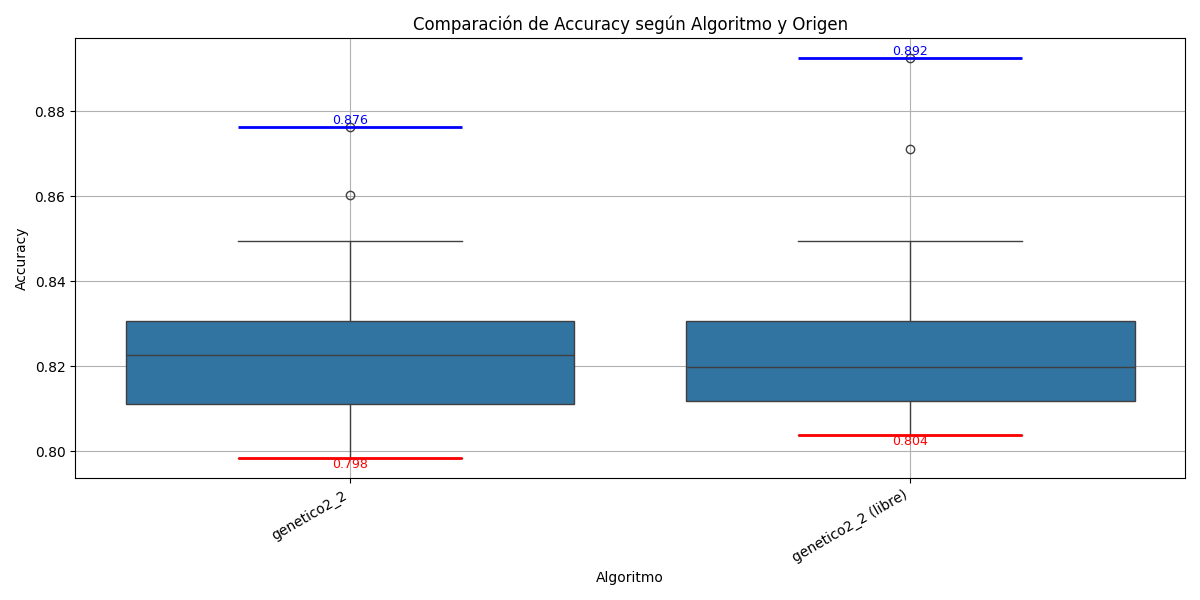
\includegraphics[width=0.9\textwidth]{imagenes/evaluaciones/libres/comparacion_gen_v2}
    \caption{Comparación de \textit{accuracy} entre el algoritmo genético v2-2 (cruce ponderado + mutación adaptativa) y su versión libre.}
    \label{fig:gen_v2_libre}
\end{figure}

En el caso del genético con cruce ponderado y mutación adaptativa (Figura~\ref{fig:gen_v2_libre}), 
los resultados son algo más matizados: la versión libre mantiene un rendimiento muy similar al de la versión rígida, 
con una leve mejora en los valores altos y un mínimo más elevado.
Esto sugiere que, aunque no siempre se observe una mejora significativa en mediana, 
la capacidad adaptativa aporta robustez adicional y mayor protección frente a ejecuciones fallidas.


\colorbox{yellow}{Falta añadir boxplot que compare el accuracy separado por cada porcentaije inicail del algoritmo genetico 2 libre.}


\begin{figure}[H]
\centering
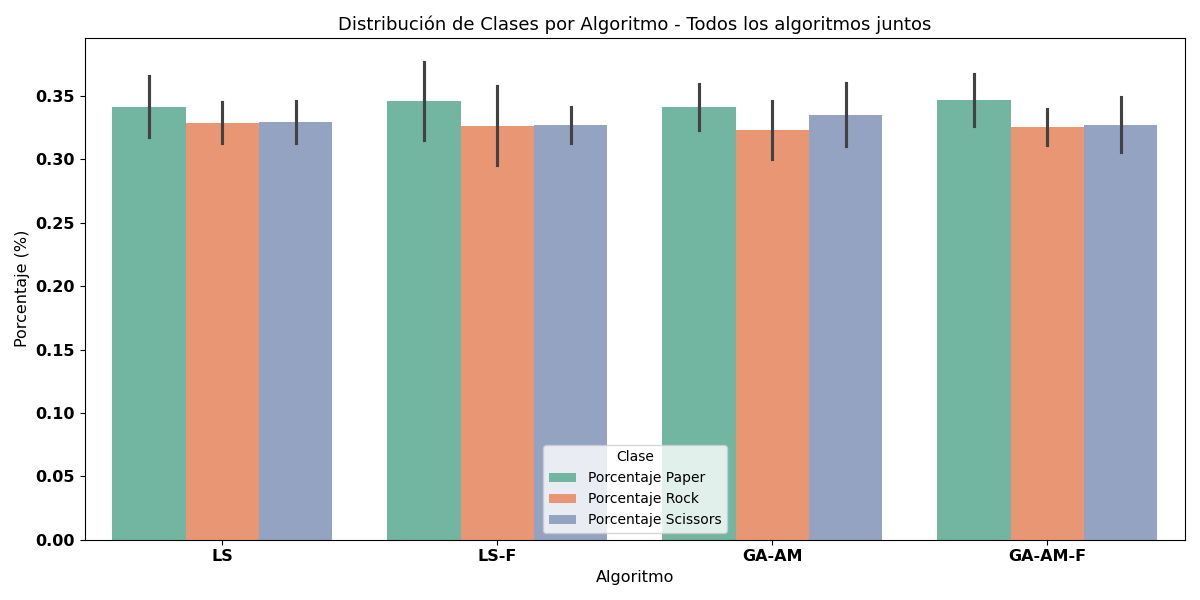
\includegraphics[width=0.9\textwidth]{imagenes/evaluaciones/libres/distribucion-clases}
\caption{Distribución de clases en los subconjuntos generados por los algoritmos estándar y libres.}
\label{fig:distribucion_libres}
\end{figure}

La Figura~\ref{fig:distribucion_libres} muestra que tanto los algoritmos estándar como sus variantes libres 
mantienen una distribución equilibrada entre las tres clases del conjunto \texttt{RPS}.
Las proporciones de \texttt{Rock}, \texttt{Paper} y \texttt{Scissors} se reproducen de forma muy similar en todos los casos, 
con únicamente pequeñas variaciones que no resultan significativas como para suponer un desbalance.

Este resultado es especialmente relevante para la validez de los experimentos, ya que confirma que los mecanismos evolutivos 
y las estrategias de ajuste del tamaño del subconjunto no introducen sesgos de clase.
La representatividad estructural del conjunto se conserva, lo cual es fundamental para garantizar una evaluación justa y equilibrada en tareas de clasificación multiclase.


\begin{figure}[H]
\centering
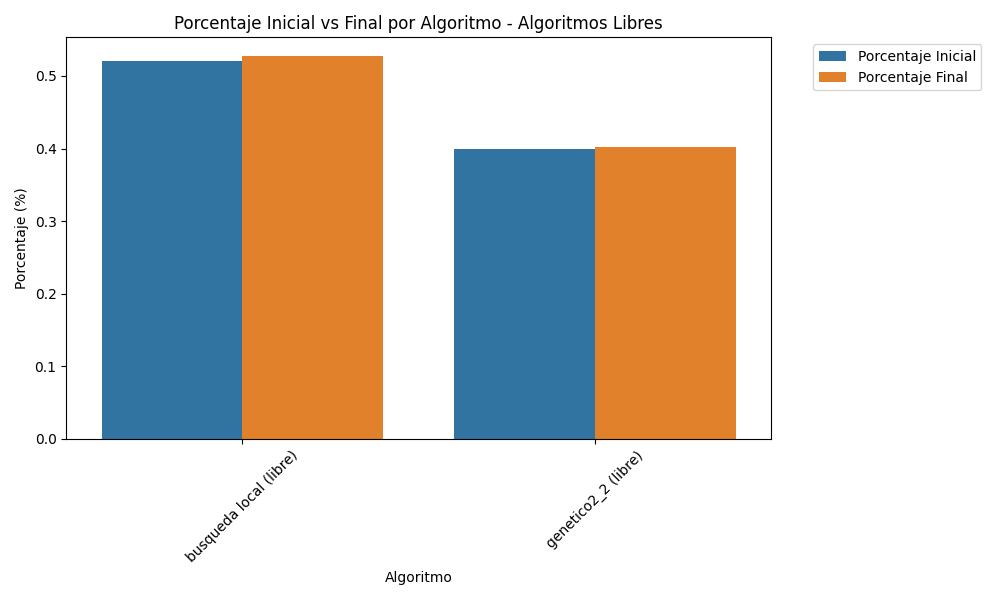
\includegraphics[width=0.9\textwidth]{imagenes/evaluaciones/libres/porcentaje-inical-vs-final-por-algoritmo}
\caption{Comparación entre porcentaje inicial y final en los algoritmos libres.}
\label{fig:porcentaje_libres_1}
\end{figure}

\begin{figure}[H]
    \centering
    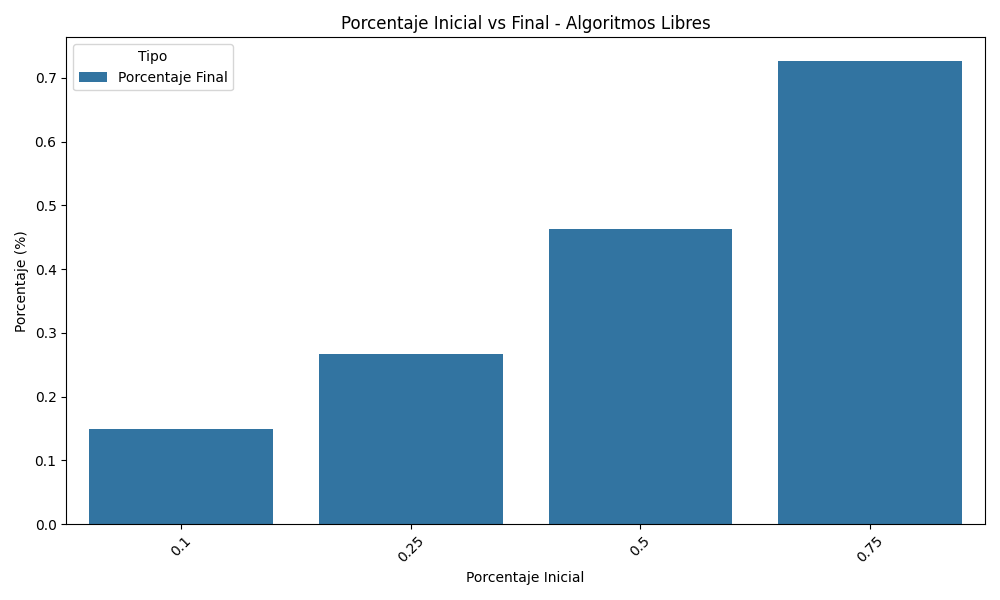
\includegraphics[width=0.9\textwidth]{imagenes/evaluaciones/libres/porcentaje-inicial-vs-final-por-pi_gev_v2.png}
    \vspace{1em}
    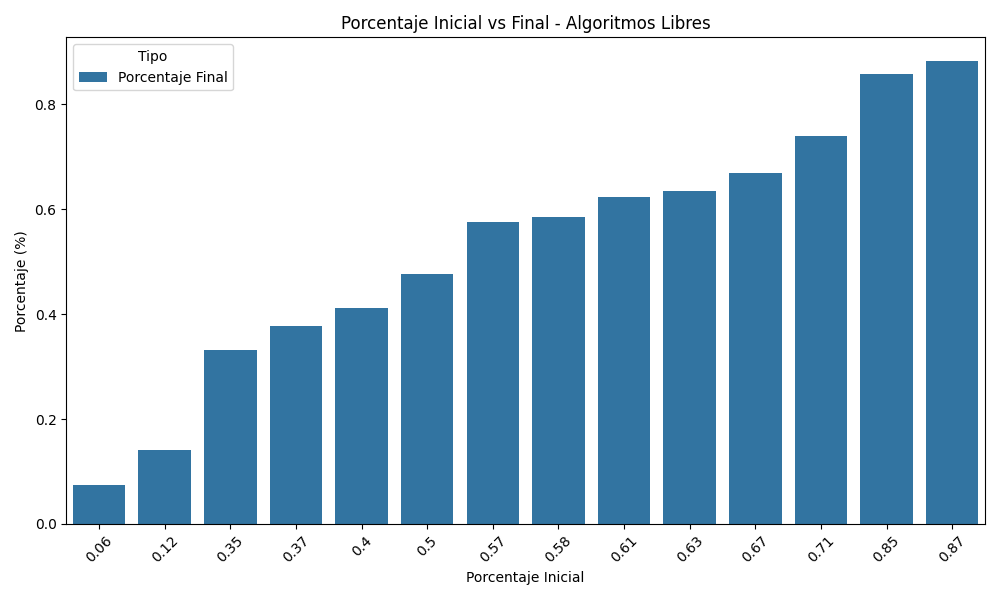
\includegraphics[width=0.9\textwidth]{imagenes/evaluaciones/libres/porcentaje-inicial-vs-final-por-pi_bl.png}
    \caption{Porcentaje final alcanzado en función del porcentaje inicial.
        Arriba: genético libre.
        Abajo: búsqueda local libre.
    }
    \label{fig:porcentaje_libres_2}
\end{figure}

Las Figuras~\ref{fig:porcentaje_libres_1} y~\ref{fig:porcentaje_libres_2} permiten analizar con mayor detalle cómo se comportan 
los algoritmos libres en términos de tamaño del subconjunto seleccionado.
En la comparación directa por algoritmo (Figura~\ref{fig:porcentaje_libres_1}), se observa que el porcentaje final tiene un leve incremento respecto al inicial.

Sin embargo, al desglosar el análisis por valores específicos del porcentaje inicial (Figura~\ref{fig:porcentaje_libres_2}), 
se aprecia un patrón más claro: cuanto mayor es el punto de partida, mayor tiende a ser también el porcentaje final alcanzado.
Esta tendencia es especialmente marcada en el caso de la búsqueda local libre, que muestra una progresión prácticamente lineal.
El algoritmo genético, en cambio, presenta un crecimiento más escalonado, pero igualmente adaptativo.

Este comportamiento sugiere que los algoritmos libres no solo adaptan la composición del subconjunto, sino también su escala, 
ajustando dinámicamente la cantidad de datos seleccionados según el entorno de búsqueda.
En general, estas versiones demuestran ser una opción más versátil y controlada, especialmente útil cuando no se conoce de antemano el tamaño óptimo del conjunto de entrenamiento.


\section{Evaluación del algoritmo memético}\label{sec:evaluacion-algoritmo-memetico}
Finalmente, se evaluó el algoritmo memético (ver \hyperref[sec:algoritmo-memetico]{Sección~\ref*{sec:algoritmo-memetico}}), 
el cual combina la evolución genética con una búsqueda local aplicada de forma probabilística sobre ciertos individuos seleccionados.
Este enfoque híbrido busca equilibrar la exploración del espacio de soluciones con una intensificación localizada, 
ofreciendo mejoras tanto en precisión como en estabilidad.


\begin{figure}[H]
\centering
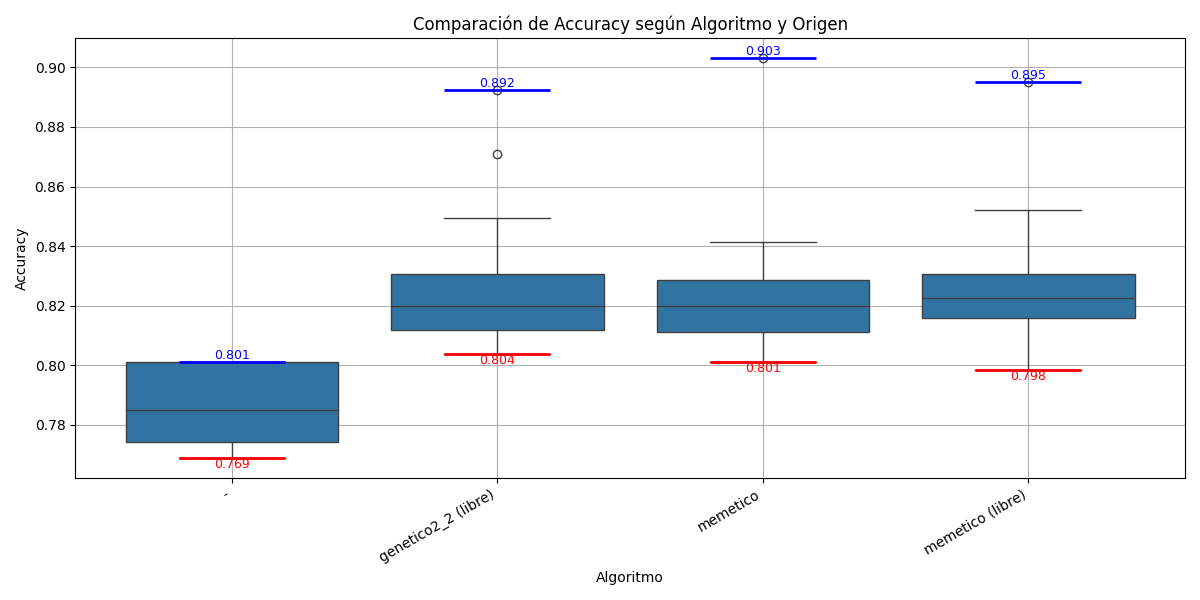
\includegraphics[width=0.9\textwidth]{imagenes/evaluaciones/comparacion-memetico}
\caption{Comparación de \textit{accuracy} entre el algoritmo memético estándar y su versión libre.}
\label{fig:memetico_comparacion}
\end{figure}

Tal como se aprecia en la Figura~\ref{fig:memetico_comparacion}, el algoritmo memético supera claramente al mejor de los enfoques genéticos 
(el Genetico Libre con Cruce Ponderado y Mutación Adaptativa), alcanzando una mediana más elevada y un valor máximo de \textit{accuracy} de hasta \textbf{0.903}.
Su distribución es más compacta, con menor dispersión hacia los valores bajos, lo que refleja una mayor consistencia entre ejecuciones.

La versión libre del memético, que incorpora también un ajuste dinámico del tamaño del subconjunto 
(ver \hyperref[subsec:memetico-libre]{Apartado~\ref*{subsec:memetico-libre}}), muestra un rendimiento muy similar al estándar, 
con una ligera reducción en el valor máximo pero una estabilidad comparable.
Esto sugiere que el componente adaptativo no penaliza la calidad de las soluciones y puede incluso aportar mayor flexibilidad en entornos más inciertos.

\begin{figure}[H]
\centering
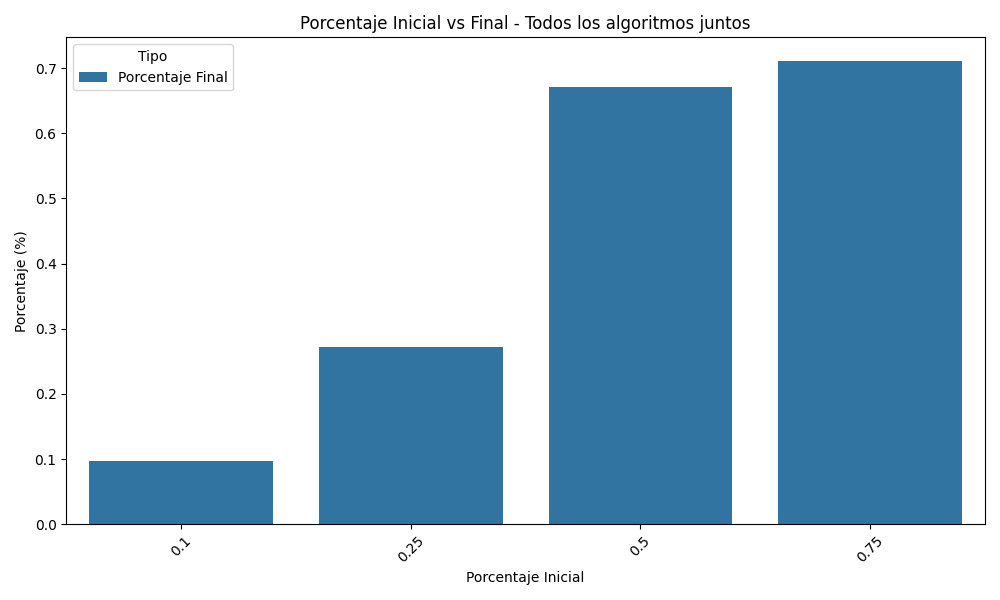
\includegraphics[width=0.9\textwidth]{imagenes/evaluaciones/libres/porcentaje-inicial-vs-final-por-pi_memetico-libre}
\caption{Porcentaje final alcanzado por el algoritmo memético libre en función del porcentaje inicial.}
\label{fig:memetico_porcentaje}
\end{figure}

En la Figura~\ref{fig:memetico_porcentaje} se observa cómo el memético libre tiende a incrementar el tamaño del subconjunto conforme aumenta el porcentaje inicial.
La curva es progresiva y cercana a la linealidad, lo que indica un comportamiento estructuralmente coherente: 
el algoritmo detecta cuándo puede beneficiarse de incluir más ejemplos y adapta su escala en consecuencia.
Este ajuste dinámico refuerza su capacidad para equilibrar rendimiento y tamaño, maximizando la eficiencia de la selección sin depender de una configuración fija.

\colorbox{yellow}{¿Añadir el párrafo de resumen?}
En resumen, tanto el memético estándar como su variante libre se consolidan como las estrategias más eficaces del estudio.
Su combinación de precisión elevada, estabilidad entre ejecuciones y capacidad adaptativa los convierte en soluciones 
especialmente robustas para tareas donde se requiere seleccionar subconjuntos representativos sin comprometer el rendimiento del modelo entrenado.


\section{Comparación final entre enfoques}\label{sec:comparacion-final-enfoques}
En esta sección se realiza una comparación conjunta entre todos los algoritmos implementados.
Se presentan boxplots y gráficos de barras que muestran la evolución del \textit{accuracy}, el porcentaje de datos utilizados y el equilibrio entre clases.

% Los algoritmos meméticos y genéticos v2/v3 (especialmente en sus versiones libres) destacan como los más eficaces, consiguiendo una reducción significativa del conjunto de entrenamiento sin penalizar la precisión.
% Además, se observa una menor varianza en sus resultados, lo que indica una mayor consistencia entre ejecuciones.

\colorbox{yellow}{Falta realizar la comparación final.}


\section{Validación con el dataset \texttt{PAINTING}}\label{sec:validacion-con-painting}
Para comprobar la robustez de los algoritmos desarrollados, se validaron los experimentos con el dataset \texttt{PAINTING},
caracterizado por una mayor complejidad visual y un número superior de clases respecto al conjunto \texttt{RPS}.
Con el fin de mantener un equilibrio entre complejidad y coste computacional, se limitaron los experimentos a los porcentajes iniciales del 25\% y 50\%,
evaluando únicamente los algoritmos más representativos.

En particular, se seleccionó el algoritmo memético, junto con su versión libre, ya que ambos habían demostrado ser los más eficaces en las pruebas anteriores.
Para establecer una referencia clara, se incluyó también los resultados obtenidos usando el 100\% del conjunto de datos, y para la compración de
\textit{accuracy} entre algoritmos también se añadió el resultado del algoritmo aleatorio.

\subsection{Comparación de \textit{accuracy} entre algoritmos}
\begin{figure}[H]
    \centering
    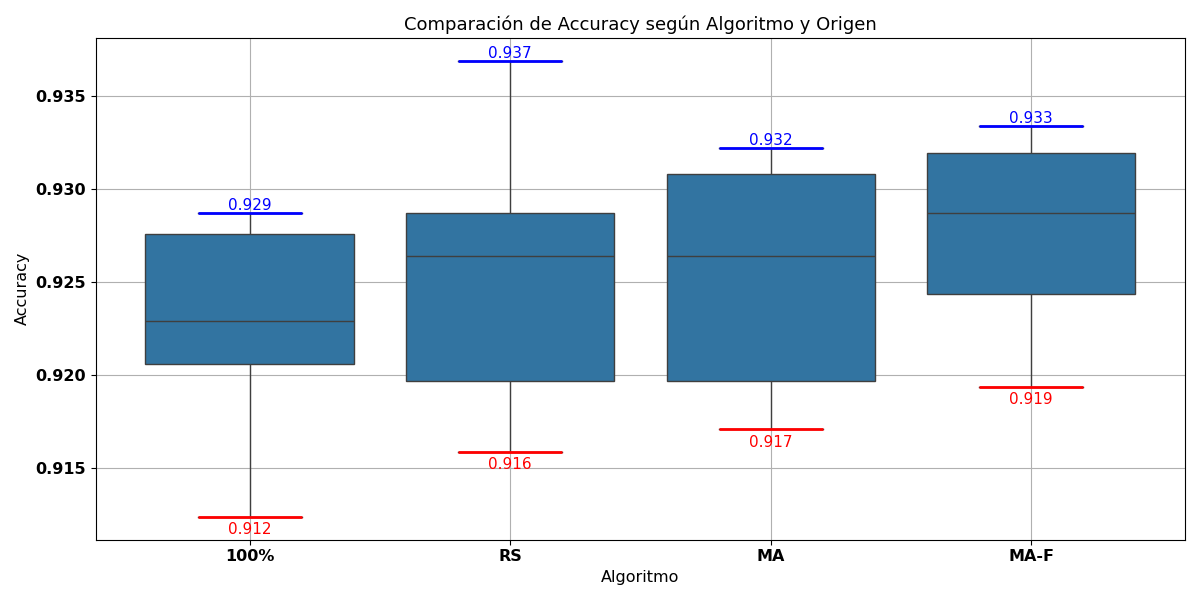
\includegraphics[width=1\textwidth]{imagenes/evaluaciones/painting/comparacion-por-algoritmo}
    \caption{Boxplot comparando resultados con el dataset \texttt{PAINTING} usando \textit{accuracy}.}
    \label{fig:comparacion-por-algoritmo}
\end{figure}

En la Figura~\ref{fig:comparacion-por-algoritmo} se comparan los valores de \textit{accuracy} obtenidos al aplicar distintos
algoritmos de selección de subconjuntos en el conjunto de datos \texttt{PAINTING}.
A simple vista, destaca el buen rendimiento de los tres enfoques meméticos frente al uso directo del 100\% del conjunto o la selección aleatoria,
lo cual es especialmente significativo al tratarse de un conjunto con alta complejidad visual y estructural.

El algoritmo memético libre obtiene el mejor rendimiento general, con una mediana que ronda el \textbf{0.927} y un valor máximo de \textbf{0.933},
superando incluso la ejecución con el 100\% de los datos, cuyo máximo se sitúa en \textbf{0.929}.
Esto no solo refuerza su capacidad de generalización, sino que demuestra que una selección optimizada puede superar a la totalidad del conjunto original,
posiblemente por eliminar ejemplos redundantes o incluso perjudiciales.

El algoritmo memético estándar también muestra una precisión elevada, con una mediana apenas inferior al libre, y un máximo de \textbf{0.931}.
Sin embargo, su varianza es ligeramente mayor, lo que sugiere que la falta de ajuste dinámico del tamaño del subconjunto puede limitar su adaptabilidad en ciertas ejecuciones.

Por otro lado, la selección aleatoria, aunque muestra valores aceptables, vuelve a confirmar su principal debilidad: la alta dispersión.
Con un mínimo de \textbf{0.916} y una mediana prácticamente idéntica a la obtenida con el uso completo del dataset, 
su comportamiento se sitúa como una referencia básica pero poco fiable.
Puede alcanzar buenos resultados, pero lo hace de forma inconsistente y sin mecanismos que garanticen estabilidad.

La ejecución con el \textbf{100\%} de los datos, utilizada como referencia absoluta, queda por debajo de las soluciones obtenidas por los algoritmos meméticos.
Esto valida empíricamente que no es la cantidad de datos, sino su calidad y representatividad, lo que determina la eficacia del entrenamiento en entornos complejos.

\colorbox{yellow}{¿Añadir el párrafo de resumen?}
En conjunto, esta comparación deja clara la superioridad de las estrategias meméticas, especialmente en su versión libre,
tanto por su rendimiento medio como por su estabilidad.
Esto refuerza la hipótesis de que los algoritmos de selección basados en evolución y búsqueda local son capaces de generar
subconjuntos más eficientes y fiables que los enfoques ingenuos o el uso total de los datos.

\subsection{Impacto del porcentaje inicial}
\begin{figure}[h]
    \centering
    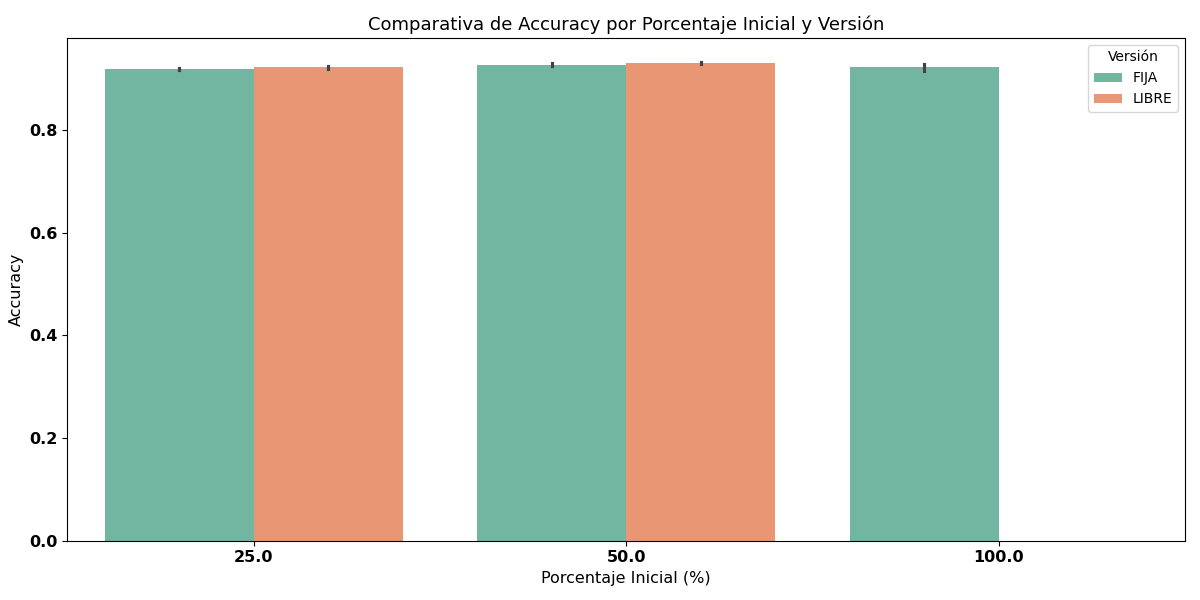
\includegraphics[width=1\textwidth]{imagenes/evaluaciones/painting/comparacion-por-porcentaje}
    \caption{Boxplot de \textit{accuracy} según el porcentaje inicial de datos.}
    \label{fig:accuracy_porcentaje_painting}
\end{figure}

La Figura~\ref{fig:accuracy_porcentaje_painting} muestra cómo varía el rendimiento del modelo (medido en términos de \textit{accuracy})
al utilizar diferentes porcentajes iniciales de datos para los algoritmos meméticos en el dataset \texttt{PAINTING}.
Lo primero que destaca es que el uso del 50\% del conjunto original no solo logra un rendimiento equiparable, sino incluso superior al uso del 100\%.
Con una mediana cercana a \textbf{0.930} y un máximo de \textbf{0.933}, este porcentaje logra un equilibrio ideal entre compresión de datos y preservación de información relevante.

Este resultado sugiere que, a partir de cierto umbral, añadir más datos no solo deja de aportar valor, sino que puede introducir ruido o redundancia.
En este caso, el entrenamiento con el 100\% de los datos exhibe mayor dispersión y un mínimo significativamente más bajo (\textbf{0.912}),
lo cual indica una mayor variabilidad entre ejecuciones y una menor estabilidad general.

Por otro lado, el uso del 25\% inicial también demuestra un rendimiento sorprendentemente competitivo,
alcanzando un máximo de \textbf{0.925}.
Sin embargo, su rango intercuartílico más estrecho (menor dispersión de los resultados) y su menor valor mínimo 
(\textbf{0.917}) evidencian una cierta fragilidad ante la reducción excesiva:
puede funcionar bien si la selección es óptima, pero el margen de error es menor.

Este comportamiento ilustra un fenómeno interesante en la reducción de datos: no existe una relación lineal entre cantidad de datos y precisión,
sino que el valor está en la calidad y representatividad del subconjunto.
El resultado más robusto refuerza la hipótesis de que existe un punto de saturación
a partir del cual la adición de ejemplos tiene un efecto marginal o incluso contraproducente en modelos convolucionales.

\colorbox{yellow}{¿Añadir el párrafo de resumen?}
En conjunto, los resultados de este apartado respaldan la viabilidad de aplicar técnicas de reducción de datos en entornos reales,
sugiriendo que con solo la mitad de los datos cuidadosamente seleccionados se puede no solo igualar,
sino superar el rendimiento de un entrenamiento exhaustivo con todo el dataset.

\subsection{Equilibrio en la distribución de clases}
\begin{figure}[h]
    \centering
    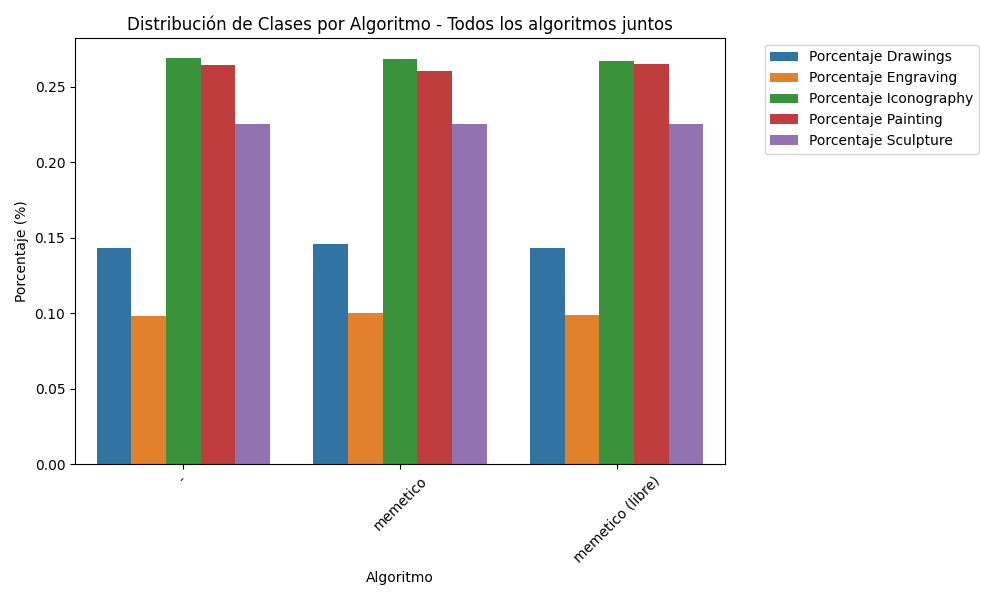
\includegraphics[width=0.9\textwidth]{imagenes/evaluaciones/painting/balance-de-clases-por-algoritmo}
    \caption{Distribución de clases seleccionadas por cada algoritmo.}
    \label{fig:balance_clases_painting}
\end{figure}

La Figura~\ref{fig:balance_clases_painting} muestra la proporción de clases preservada por cada algoritmo durante el proceso de reducción.
Se observa que tanto el algoritmo memético estándar como el libre mantienen una distribución prácticamente idéntica a la original,
sin introducir sesgos estructurales.

Las clases mayoritarias (\texttt{Iconography}, \texttt{Painting} y \texttt{Sculpture}) se mantienen consistentes en su proporción,
al igual que las clases minoritarias (\texttt{Drawings} y \texttt{Engraving}).
Esta conservación sugiere que el proceso de selección no actúa de forma aleatoria ni ciega,
sino que incorpora implícitamente una presión hacia la diversidad, lo cual es clave en problemas multiclase.

\subsection{Evolución del tamaño del subconjunto}
\begin{figure}[H]
    \centering
    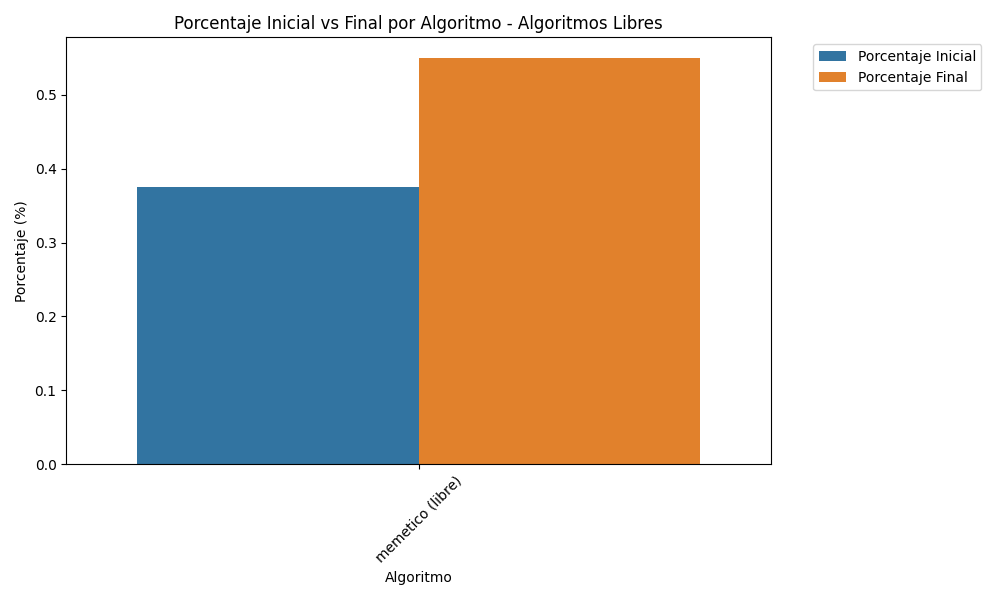
\includegraphics[width=0.9\textwidth]{imagenes/evaluaciones/painting/porcentaje-inical-vs-final-por-algoritmo}
    \vspace{1em}
    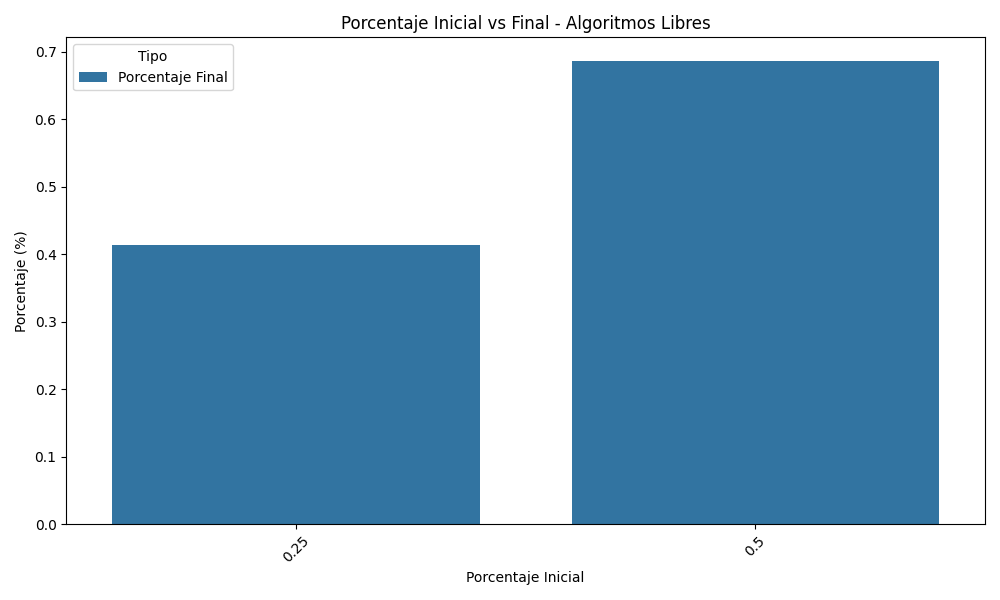
\includegraphics[width=0.9\textwidth]{imagenes/evaluaciones/painting/porcentaje-inicial-vs-final-por-pi}
    \caption{Evolución del tamaño del subconjunto seleccionado por los algoritmos libres.
        Arriba: comparación por algoritmo.
        Abajo: evolución según el porcentaje inicial.
    }
    \label{fig:evolucion_porcentaje_libre}
\end{figure}

En la Figura~\ref{fig:evolucion_porcentaje_libre} se analiza cómo evolucionó el tamaño de los subconjuntos seleccionados por los algoritmos libres respecto al valor inicial.
Se observa que el algoritmo memético libre tiende a incrementar el porcentaje de imágenes seleccionadas durante el proceso evolutivo.

Este comportamiento adaptativo pone de manifiesto la capacidad del algoritmo para ajustar dinámicamente la escala de la solución en función de la complejidad del problema.
A diferencia de enfoques con tamaño fijo, el algoritmo libre no solo decide qué ejemplos seleccionar, sino también cuántos,
ampliando el conjunto cuando detecta que puede mejorar el rendimiento sin incurrir en sobreajuste.

Además, se observa que al partir del 25\% inicial, el algoritmo tiende a aumentar el tamaño del subconjunto hasta un 16,35\% adicional,
en cambio, al partir del 50\% inicial, el crecimiento es mayor, alcanzando un 18,69\% adicional~\footnote{Porcentajes exactos sacados de la tabla de resultados.}.
Este hecho puede sugerir una cierta prudencia evolutiva: el algoritmo no se expande indiscriminadamente,
sino que responde a señales de mejora en el proceso de evaluación.
Este mecanismo emergente refuerza la versatilidad del enfoque libre, que no solo busca soluciones de alta calidad,
sino que lo hace optimizando también el volumen de datos utilizados.


\bigskip

\subsection*{Síntesis final de la validación con \texttt{PAINTING}}
Los resultados obtenidos con el dataset \texttt{PAINTING} confirman la solidez y capacidad de generalización de los algoritmos desarrollados.
Tanto el enfoque memético estándar como, especialmente, su versión libre, lograron mantener un rendimiento competitivo en un entorno más complejo y con mayor número de clases.

Se evidenció que es posible superar el rendimiento del conjunto completo de entrenamiento utilizando únicamente un subconjunto bien seleccionado,
reduciendo significativamente el volumen de datos sin comprometer la precisión.
Además, los algoritmos meméticos demostraron preservar el equilibrio entre clases y adaptarse dinámicamente al tamaño del subconjunto,
lo que constituye una ventaja clave en tareas reales donde no siempre se dispone de datasets perfectamente balanceados ni completos.

En conjunto, esta validación externa no solo refuerza las conclusiones obtenidas con \texttt{RPS},
sino que demuestra que el uso de técnicas evolutivas, y en particular las variantes libres, puede ser una alternativa eficaz,
escalable y controlable frente a la selección masiva o aleatoria de datos en procesos de entrenamiento profundo.
